\documentclass[a4paper, 12pt]{beamer}

\usetheme{metropolis}
% Paquetes necesarios
\usepackage[utf8]{inputenc}
\usepackage[T1]{fontenc}
\usepackage{helvet}
\usepackage[spanish]{babel}
\usepackage{amsmath, amssymb, amsfonts, amsthm, amssymb}
\usepackage{cite}
\usepackage{listings}
\usepackage{color}
\usepackage{graphicx}
\usepackage{xcolor}
\definecolor{dorado}{RGB}{239, 184, 16}
\definecolor{plata}{RGB}{192, 192, 192}
\definecolor{verde}{RGB}{40, 114, 51}
\definecolor{rojo}{RGB}{139, 0, 0}
\definecolor{amarillo}{RGB}{229, 190, 1}
\definecolor{azul}{RGB}{9, 108, 138}
% Información del título
\title{\textcolor{dorado}{Hwent}\textcolor{plata}{-pro++}}
\subtitle{Proyecto de Programación II. Presentación de la expansión.}
\author{Melissa Maureen Sales Brito}
\institute{MatCom}
\date{}

% Contenido de la presentación
\begin{document}

\maketitle

\begin{frame}{\textcolor{plata}{Índice}}
\vspace{8pt}
\setcounter{tocdepth}{2}
\tableofcontents
\end{frame}

\section{Introducción}

\begin{frame}{\textcolor{plata}{Introducción: ¿Expansión?}}
En esta \textit{nueva fase} hemos desarrollado un \textbf{Lenguaje Específico de Dominio} (DSL) que permitirá a los jugadores crear sus propias cartas y efectos personalizados. Este DSL será interpretado no solo siguiendo las reglas establecidas del juego, sino que tambien ofrece flexibilidad para que la imaginacion de los jugadores no tenga límites. A través de esta herramienta, buscamos enriquecer la experiencia de juego, fomentando la creatividad y llevando la magia de Hogwarts a nuevas alturas.
\end{frame}

\section{DSL generalidades}
\subsection{Creando un nuevo efecto}
\begin{frame}{\textcolor{plata}{DSL: efecto}}\
effect\\
\{\\
	\hspace{1cm}  Name: \small \texttt{nombre del efecto (ej: \textbf{"Robar"})},\\
	\hspace{1cm}  Params: \{ \texttt{parámetros que recibe el efecto} \},\\
	\hspace{1cm}  Action: (\small \texttt{parámetros de la función}) => \{ \texttt{cuerpo} \};\\
\}\\
\vspace{0.6cm}
\begin{itemize}
\item Params: parámetros que recibe el efecto. Son opcionales y cada parámetro se recibe asociado a su tipo (\textbf{Number}, \textbf{Sring}, \textbf{Bool}).
\end{itemize}
\end{frame}

\begin{frame}{\textcolor{plata}{DSL: efecto}}\
\begin{itemize}
\item Action: 
\begin{itemize}
\item Se definen expícitamente dos prámetros. El primero en una lista que objetivos (cartas) y el segundo es un objeto contexto que representa el estado del juego. \texttt{Ej: (targets, context) => \{...\}}
\item El cuerpo consiste en las instrucciones que desencadena el efecto para su funcionamiento.
\end{itemize}
\end{itemize}
\end{frame}

\begin{frame}{\textcolor{plata}{DSL: nota}}\
\textbf{Nota:} debe recordar que el correcto funcionamiento de su efecto lo determina entre otros factores, que este sea programado según la lógica del juego. Las funciones \texttt{Push, Add, SendBottom} solo añaden un elemento a una lista. Durante el juego, al jugar una carta se activa inmediatamente su efecto como se explica en la primera fase del proyecto. La función de un efecto se ejecuta línea por línea, de forma que si dada una carta, que obtines mediante la lista de objetivo o a través del contexto, añades esta a una nueva lista, y luego sigue la linea que emplea el Remove (o no), puede que reubicarla desencadene instrucciones donde termina eligiendose a sí misma.
\end{frame}

\begin{frame}{\textcolor{plata}{DSL: nota}}\
\texttt{Ej: dada una carta cuyo efecto es obtener las cartas del mazo propio con poder igual a 7, luego jugarlas en el campo y posteriormente removerlas del mazo. Al jugar las cartas con poder igual a 7 se activan sus efectos como parte de la acción de añadirlas, esto puede ocasionar que por ejemplo una de estas cartas tenga el efecto de robar una carta aleatoria del mazo, de esta forma dicha carta puede ser una de las que recientemente se han añadido al campo, pero como aún no se ejecuta la linea de remover las cartas obtenidas del mazo, el juego se paraliza con un error en tiempo de ejecución.}
\end{frame}

\begin{frame}{\textcolor{plata}{DSL: contexto}}\
Como jugador con la capacidad de crear tienes acceso a:
\begin{itemize}
\item La mano de un jugador.
\item El campo de un jugador. Un campo se define como el conjunto de filas (M,R,S) de un jugador sin incluir la celda especial de aumento por fila.
\item El cementerio de un jugador.
\item El mazo de un jugador.
\item El tablero de un jugador. Se define como el cojunto de los campos de juego.
\item La zona de climas.
\item Las celdas de aumento de un jugador.
\end{itemize}
\end{frame}

\subsection{Creando una carta}
\begin{frame}{\textcolor{plata}{DSL: carta}}
card\\
\{\\
\hspace{1cm} Type: \texttt{tipo de la carta(definido)},\\
\hspace{1cm} Name: \texttt{nombre de la carta, ej:"Hagrid"},\\
\hspace{1cm} Faction: \texttt{facción de la carta(definida)},\\
\hspace{1cm} Power: \texttt{cantidad de poder de la carta},\\
\hspace{1cm} Range: [ \texttt{rangos} ],\\
\hspace{1cm} OnActivation: [ \texttt{efectos} ]\\
\}
\end{frame}

\begin{frame}{\textcolor{plata}{DSL: carta}}
\begin{itemize}
\item Tipos definidos: \textbf{"Oro", "Plata", "Lider", "Clima", "Aumento", "Despeje"}. Se añade Despeje dado que no existe un campo en card que particularice el tipo Clima.
\item Facciones definidas: \textbf{"Gryffindor", "Slytherin"}, ambas facciones estan equipadas desde la primera fase; se agregan \textbf{"Ravenclaw" , "Hufflepuff"} que solo cuentan con las cartas neutrales. La facción de las cartas especiales será ignorada.
\item El poder es una cantidad entera que será ignorada en el caso de las cartas especiales.
\end{itemize}
\end{frame}

\begin{frame}{\textcolor{plata}{DSL: carta}}
\begin{itemize}
\item Los rangos son: \textbf{"Melee", "Ranged", "Siege"}. En el caso del tipo Aumento, Lider y Despeje el rango es ignorado según la definición de la primera fase del proyecto; el tipo clima adopta el primer rango declarado.
\end{itemize}
\texttt{Declaración de efecto:}\\
\{\\
\hspace{1cm} Effect: \{ \texttt{cuerpo} \},\\
\hspace{1cm} Selector: \{ \texttt{cuerpo} \},\\
\hspace{1cm} PostAction: \{ \texttt{otra declaracion de efecto} \}\\
\}
\end{frame}

\begin{frame}{\textcolor{plata}{DSL: carta}}
\texttt{Effect}\\
\begin{itemize}
\item Definición:\\
Effect:\\
\{
\hspace{1cm} Name: \{ \texttt{nombre de un efecto definido}\},\\
\hspace{1cm} \texttt{parámetros(opcionales) como propiedades diferentes, ej:Amount:5}\\
\},
\item Azúcar sintáctica si el efecto no requiere parámetros:
Type: \texttt{nombre del efecto},\\
ó\\
Effect: \texttt{nombre del efecto},
\end{itemize}
\end{frame}

\begin{frame}{\textcolor{plata}{DSL: carta}}
\texttt{Selector}\\
Selector:\\
\{\\
\hspace{1cm} Source: \texttt{fuente, ej:"field"},\\
\hspace{1cm} Single: \texttt{valor booleano que indica si solo se toma un objetivo, ej: true},\\
\hspace{1cm} Predicate: (\texttt{identificador de la carta}) => \texttt{instrucción booleana para selecionar la carta}\\
\},
\end{frame}

\begin{frame}{\textcolor{plata}{DSL: carta}}
\texttt{Selector}\\
\begin{itemize}
\item Las fuentes definidas son:  \textbf{"board", "weatherZone", "hand", "graveyard", "deck", "field", "boosterCells"} para referirse a el tablero, zona de climas, mano, cementerio, mazo, campo y celdas de aumento propios, respectivamente, en el caso de las fuentes no comunes se agrega "other" como prefijo de la fuente \texttt{ej:"otherHand"}.
\end{itemize}
\end{frame}

\section{UI/particularidades}
\begin{frame}{\textcolor{plata}{Opción Personalizar agregada}}
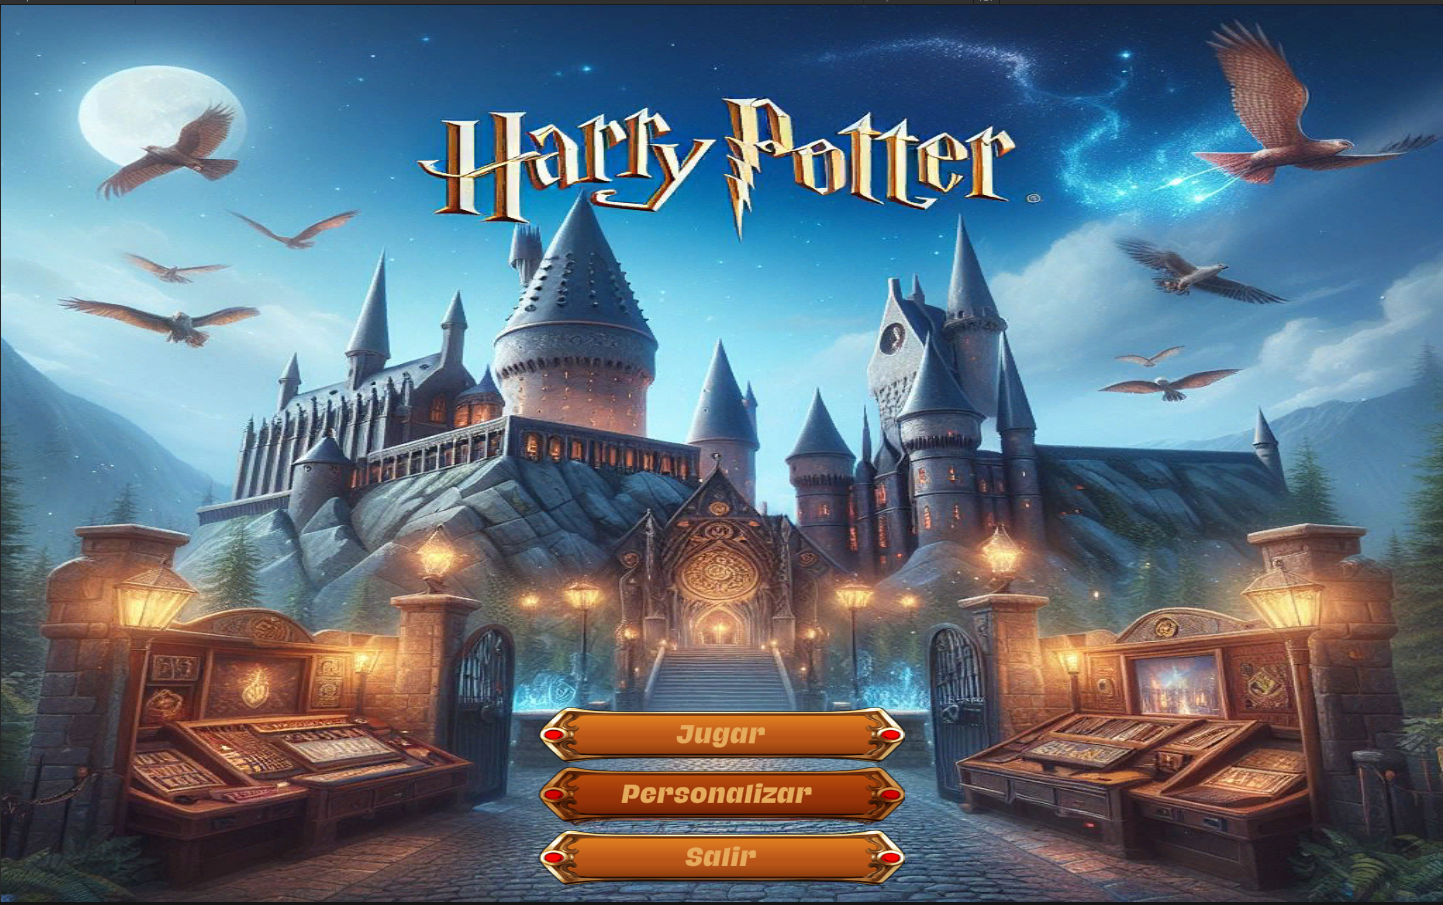
\includegraphics[scale = 0.2]{images/image10.png}
\end{frame}

\begin{frame}{\textcolor{plata}{Editor para la creación de efectos y cartas}}
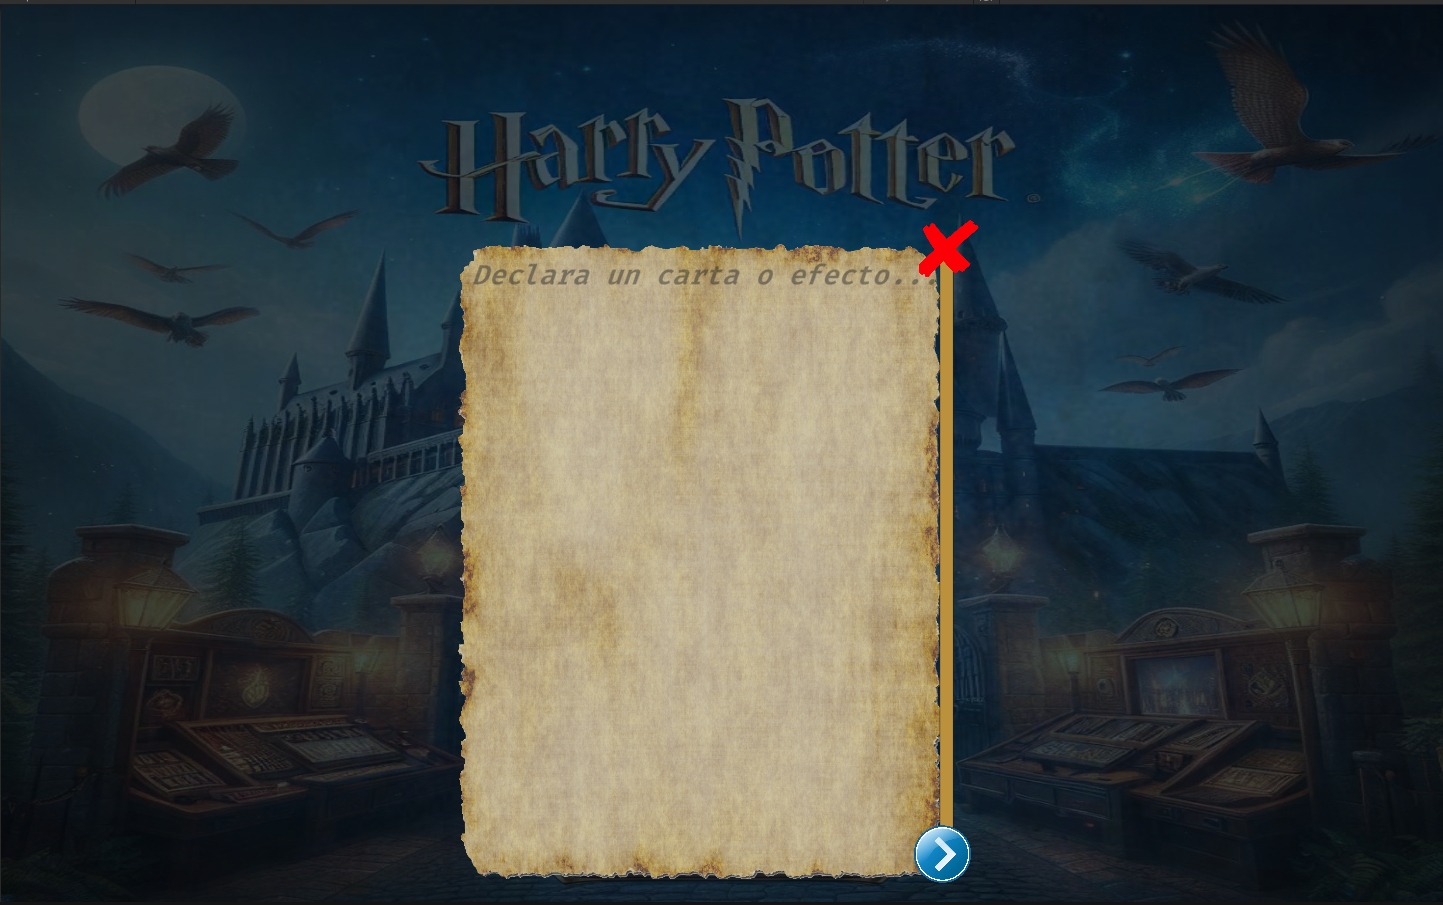
\includegraphics[scale = 0.2]{images/image11.png}
\end{frame}

\begin{frame}{\textcolor{plata}{Declaración de efecto}}
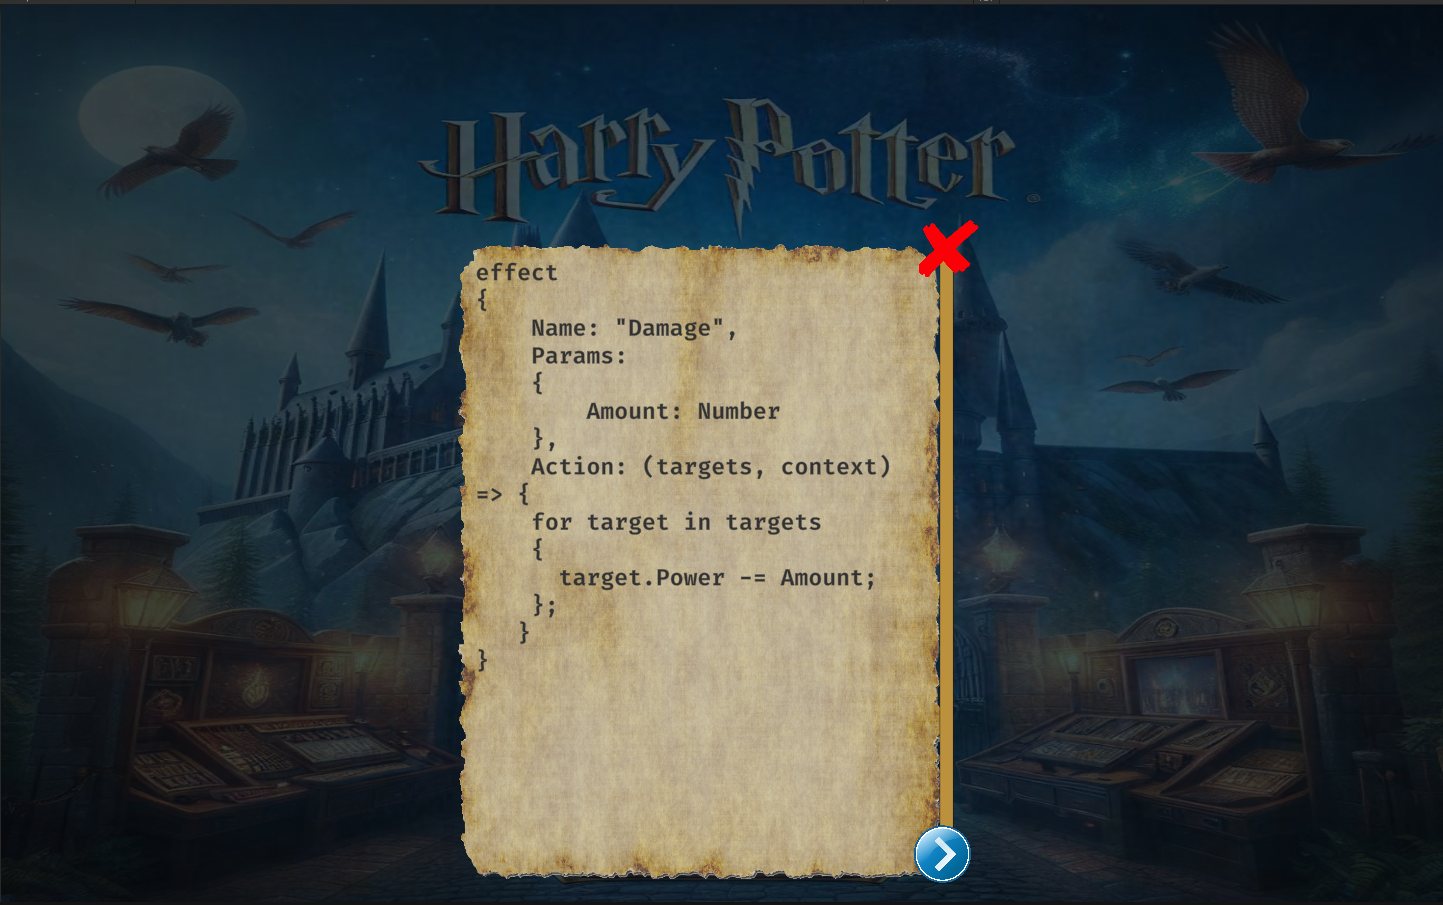
\includegraphics[scale = 0.2]{images/image12.png}
\end{frame}

\begin{frame}{\textcolor{plata}{Ventana de Error}}
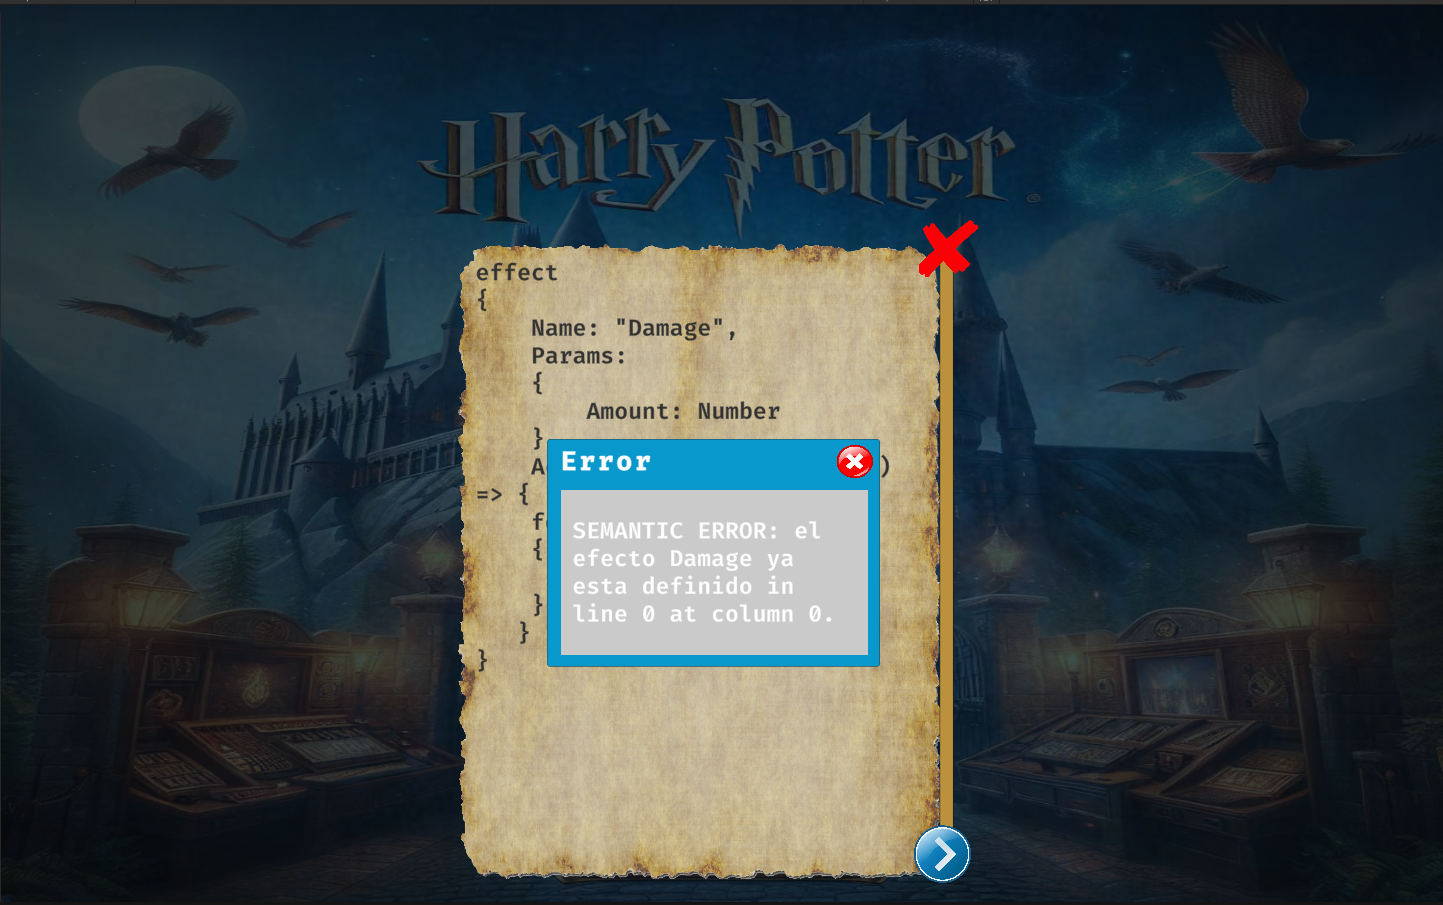
\includegraphics[scale = 0.2]{images/image13.png}
\end{frame}

\begin{frame}{\textcolor{plata}{Facciones agregadas}}
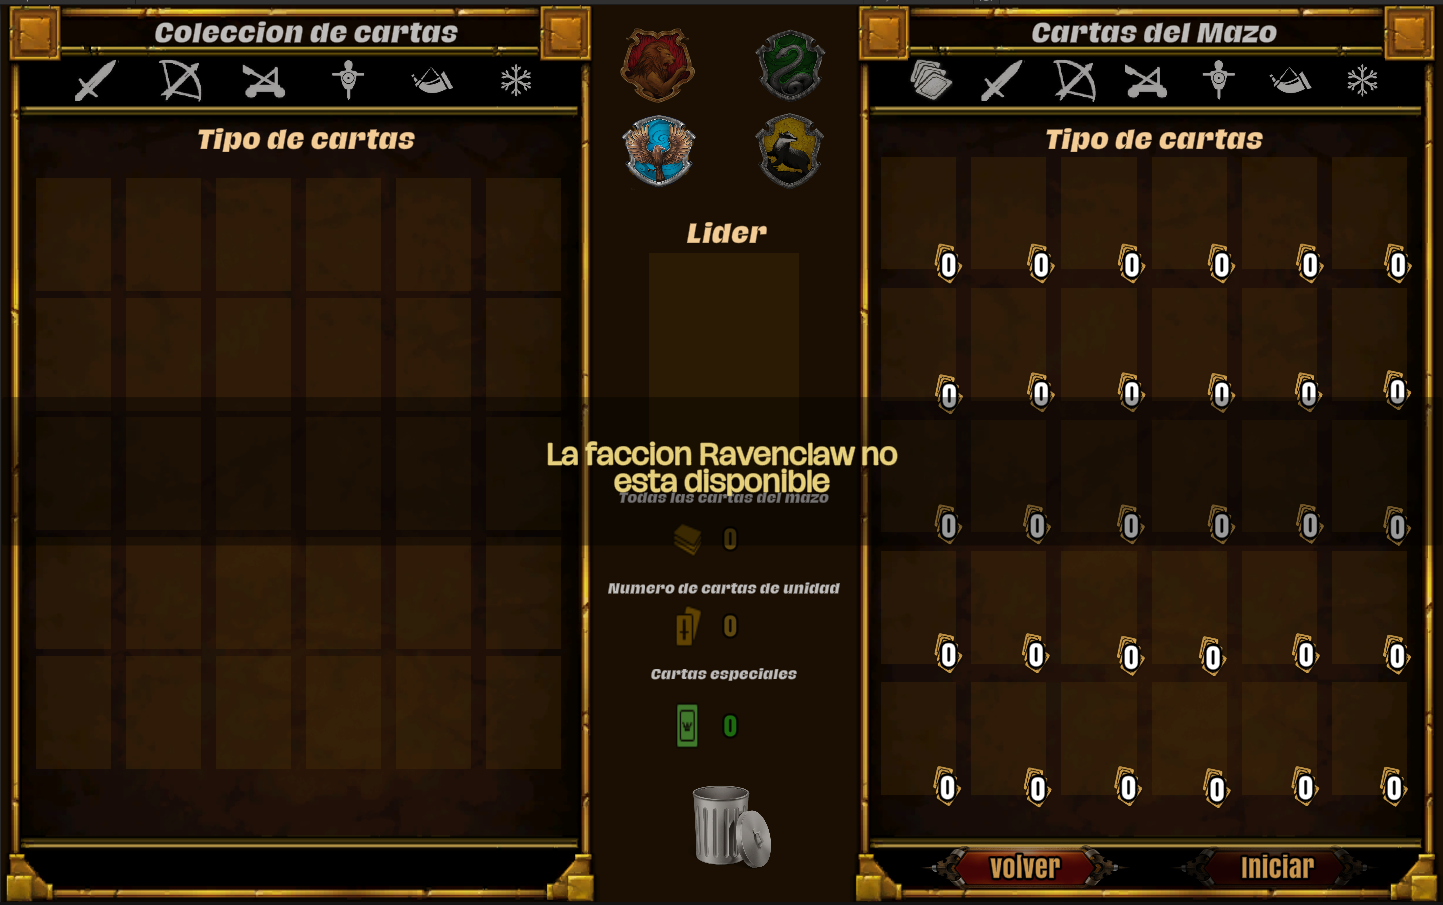
\includegraphics[scale = 0.2]{images/image14.png}\\
\begin{tiny}
Nota: se permite la creación de líderes; las facciones Ravenclaw y Hufflepuff solo son disponibles si crea al menos un líder para la faccion. Si crea un nuevo líder se escogerá como representante uno aleatorio.
\end{tiny} 
\end{frame}

\end{document}